\chapter{Функционал пользователя группы <<\gloss{auth_user}>>.}

    \section{Общие элементы страниц}
        \subsection{Главное меню}
            
            См. рис. \ref{fig:auth_main_menu}

            Все то же, что у неавторизованного пользователя (см.\ref{sec:baseitems_main_meu}), 
            плюс пункт <<профиль пользователя>> со следующими элементами:
            
            \begin{enumerate}
                \item ФИО пользователя.
                \item Количество баллов.
            \end{enumerate}


        \begin{figure}
            \center
            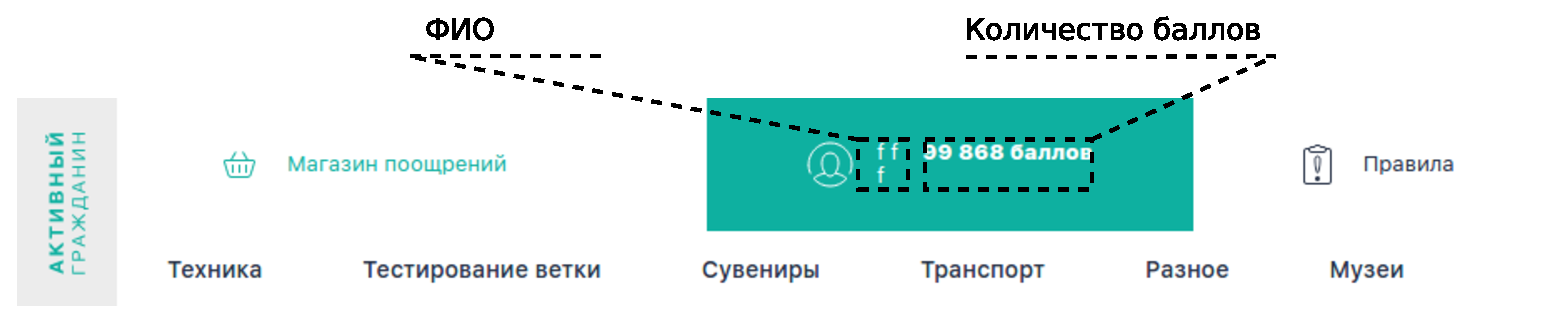
\includegraphics[width=170mm]{04_auth_funcs/figures/01.eps}
            \caption{Главное меню авторизованного пользователя}
            \label{fig:auth_main_menu}
        \end{figure}
        
        \subsection{Фильтр по цене и интересам}

            См. рис. \ref{fig:auth_filter}

            Вместо ссылки на авторизацию (см. \ref{sec:noauth_filter_points}) появляется дополнительная вкладка
            <<у меня N баллов>>, задающая диапазон фильтрации товаров по баллам.
            
            \begin{enumerate}
                \item По умолчанию выставляется число баллов от нуля до количества, которое есть у пользователя.
                \item Есть элемент, позволяющий фильтровать товары независимо от количества баллов у пользователя <<все баллы>>.
                \item Остальные элементы управления задают диапазоны между порядками цен (0$\dots$10, 11$\dots$100 и т.д.).
                \item Выбрать можно только один диапазон.
            \end{enumerate}

            
            \begin{figure}
                \center
                
\includegraphics[width=170mm]{04_auth_funcs/figures/02.eps}
                \caption{Фильтр по количеству баллов}
                \label{fig:auth_filter}
            \end{figure}
        
        \subsection{Тизер товара}

            См. рис. \ref{fig:auth_tizer}
        
            Единственное отличие от тизера товара для неавторизованного пользователя (см. \ref{sec:noauth_tizer})
            --- это активная ссылка <<желание>>.
            \begin{enumerate}
                \item Товар можно добавить в <<мои желания>> кликом по <<сердечку>>
                \item Сердечко товара, добавленного в <<мои желания>> заливается красным.
                \item Товар, добавленный в <<мои желания>> появляется в соответствующем разделе (см.\ref{sec:auth_my_wishes}).
            \end{enumerate}

        
            \begin{figure}
                \center
                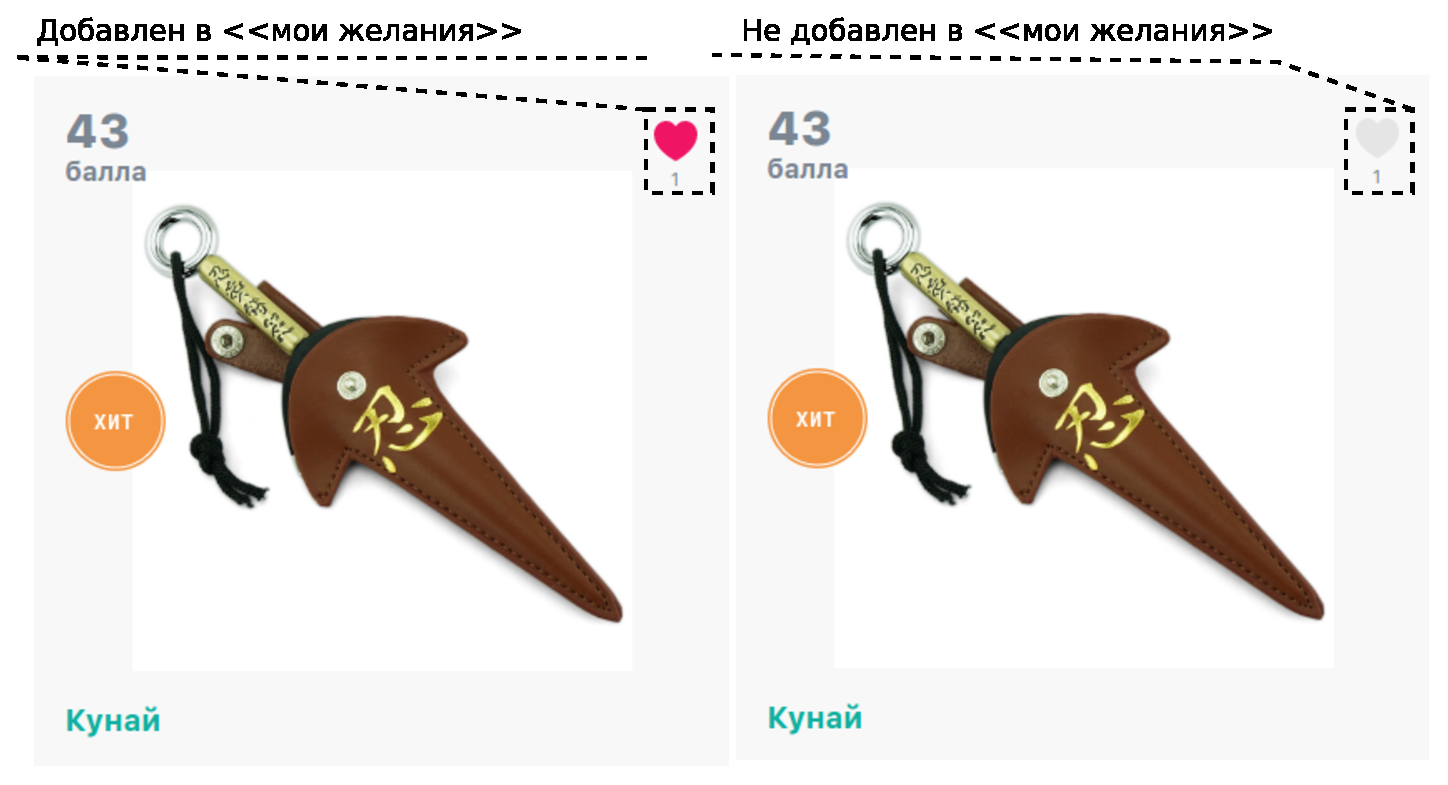
\includegraphics[width=170mm]{04_auth_funcs/figures/03.eps}
                \caption{Тизер товара для авторизованного пользователя.}
                \label{fig:auth_tizer}
            \end{figure}
        
        
    \section{Главная страница}
        \subsection{Банер слайдер}
        
            См. рис. \ref{fig:auth_slide_goods}

            Единственное отличие от слайда-товара для неавторизованного пользователя (см. \ref{sec:noauth_slide_goods})
            --- это активная ссылка <<желание>>.
            
            \begin{enumerate}
                \item Товар можно добавить в <<мои желания>> кликом по <<сердечку>>
                \item Сердечко товара, добавленного в <<мои желания>> заливается красным.
                \item Товар, добавленный в <<мои желания>> появляется в соответствующем разделе (см.\ref{sec:auth_my_wishes}).
            \end{enumerate}
            
            \begin{figure}
                \center
                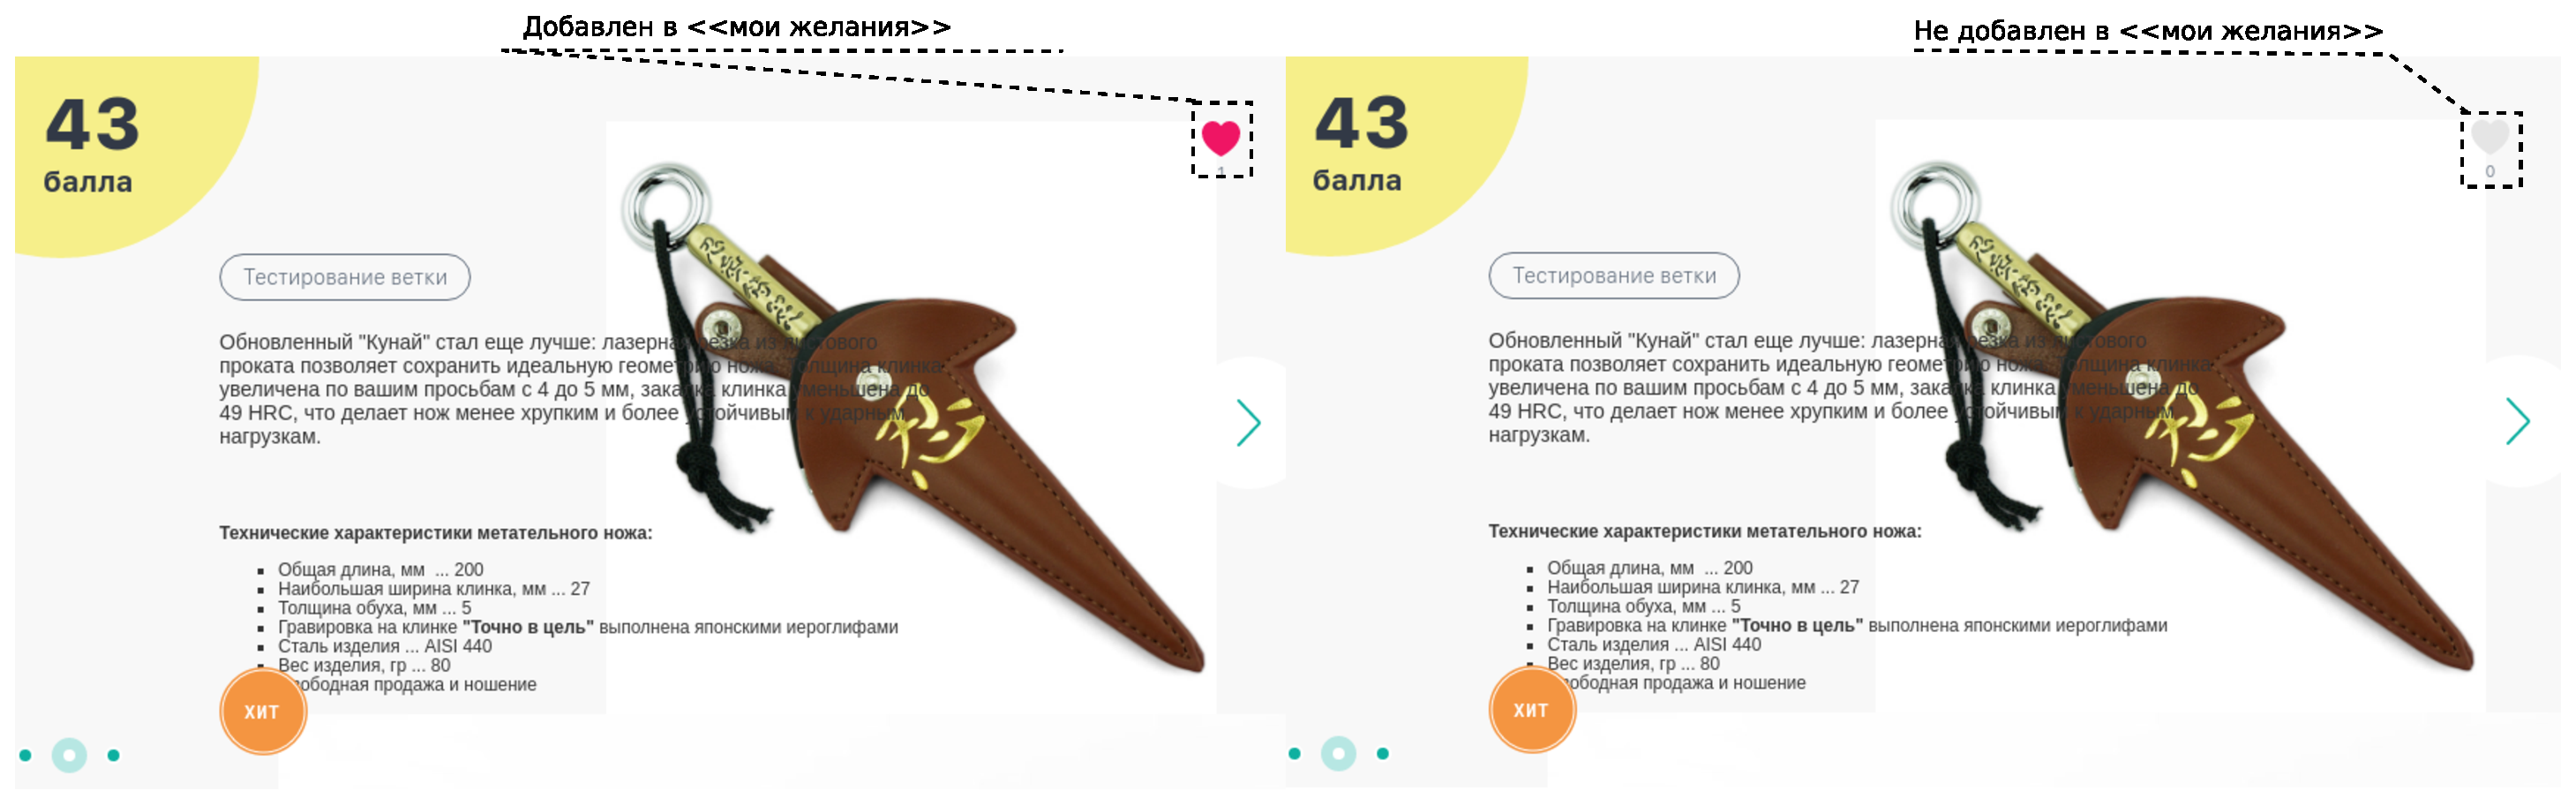
\includegraphics[width=170mm]{04_auth_funcs/figures/04.eps}
                \caption{Слайд-товар для авторизованного пользователя.}
                \label{fig:auth_slide_goods}
            \end{figure}
        
        
     \section{Карточка товара}

        См. рис. \ref{fig:auth_goods_cart}
     
        \subsection{Склад выдачи}
        \subsection{Количество заказываемых единиц}
        \subsection{Кнопка заказа}
        \subsection{Форма подтверждения заказа}
        \subsection{Отзывы}

            См. рис. \ref{fig:auth_goods_cart_otz}
        
            \subsubsection{Форма добавления отзыва}
                \paragraph{Сообщение}
                \paragraph{Оценка}

            \begin{figure}
                \center
                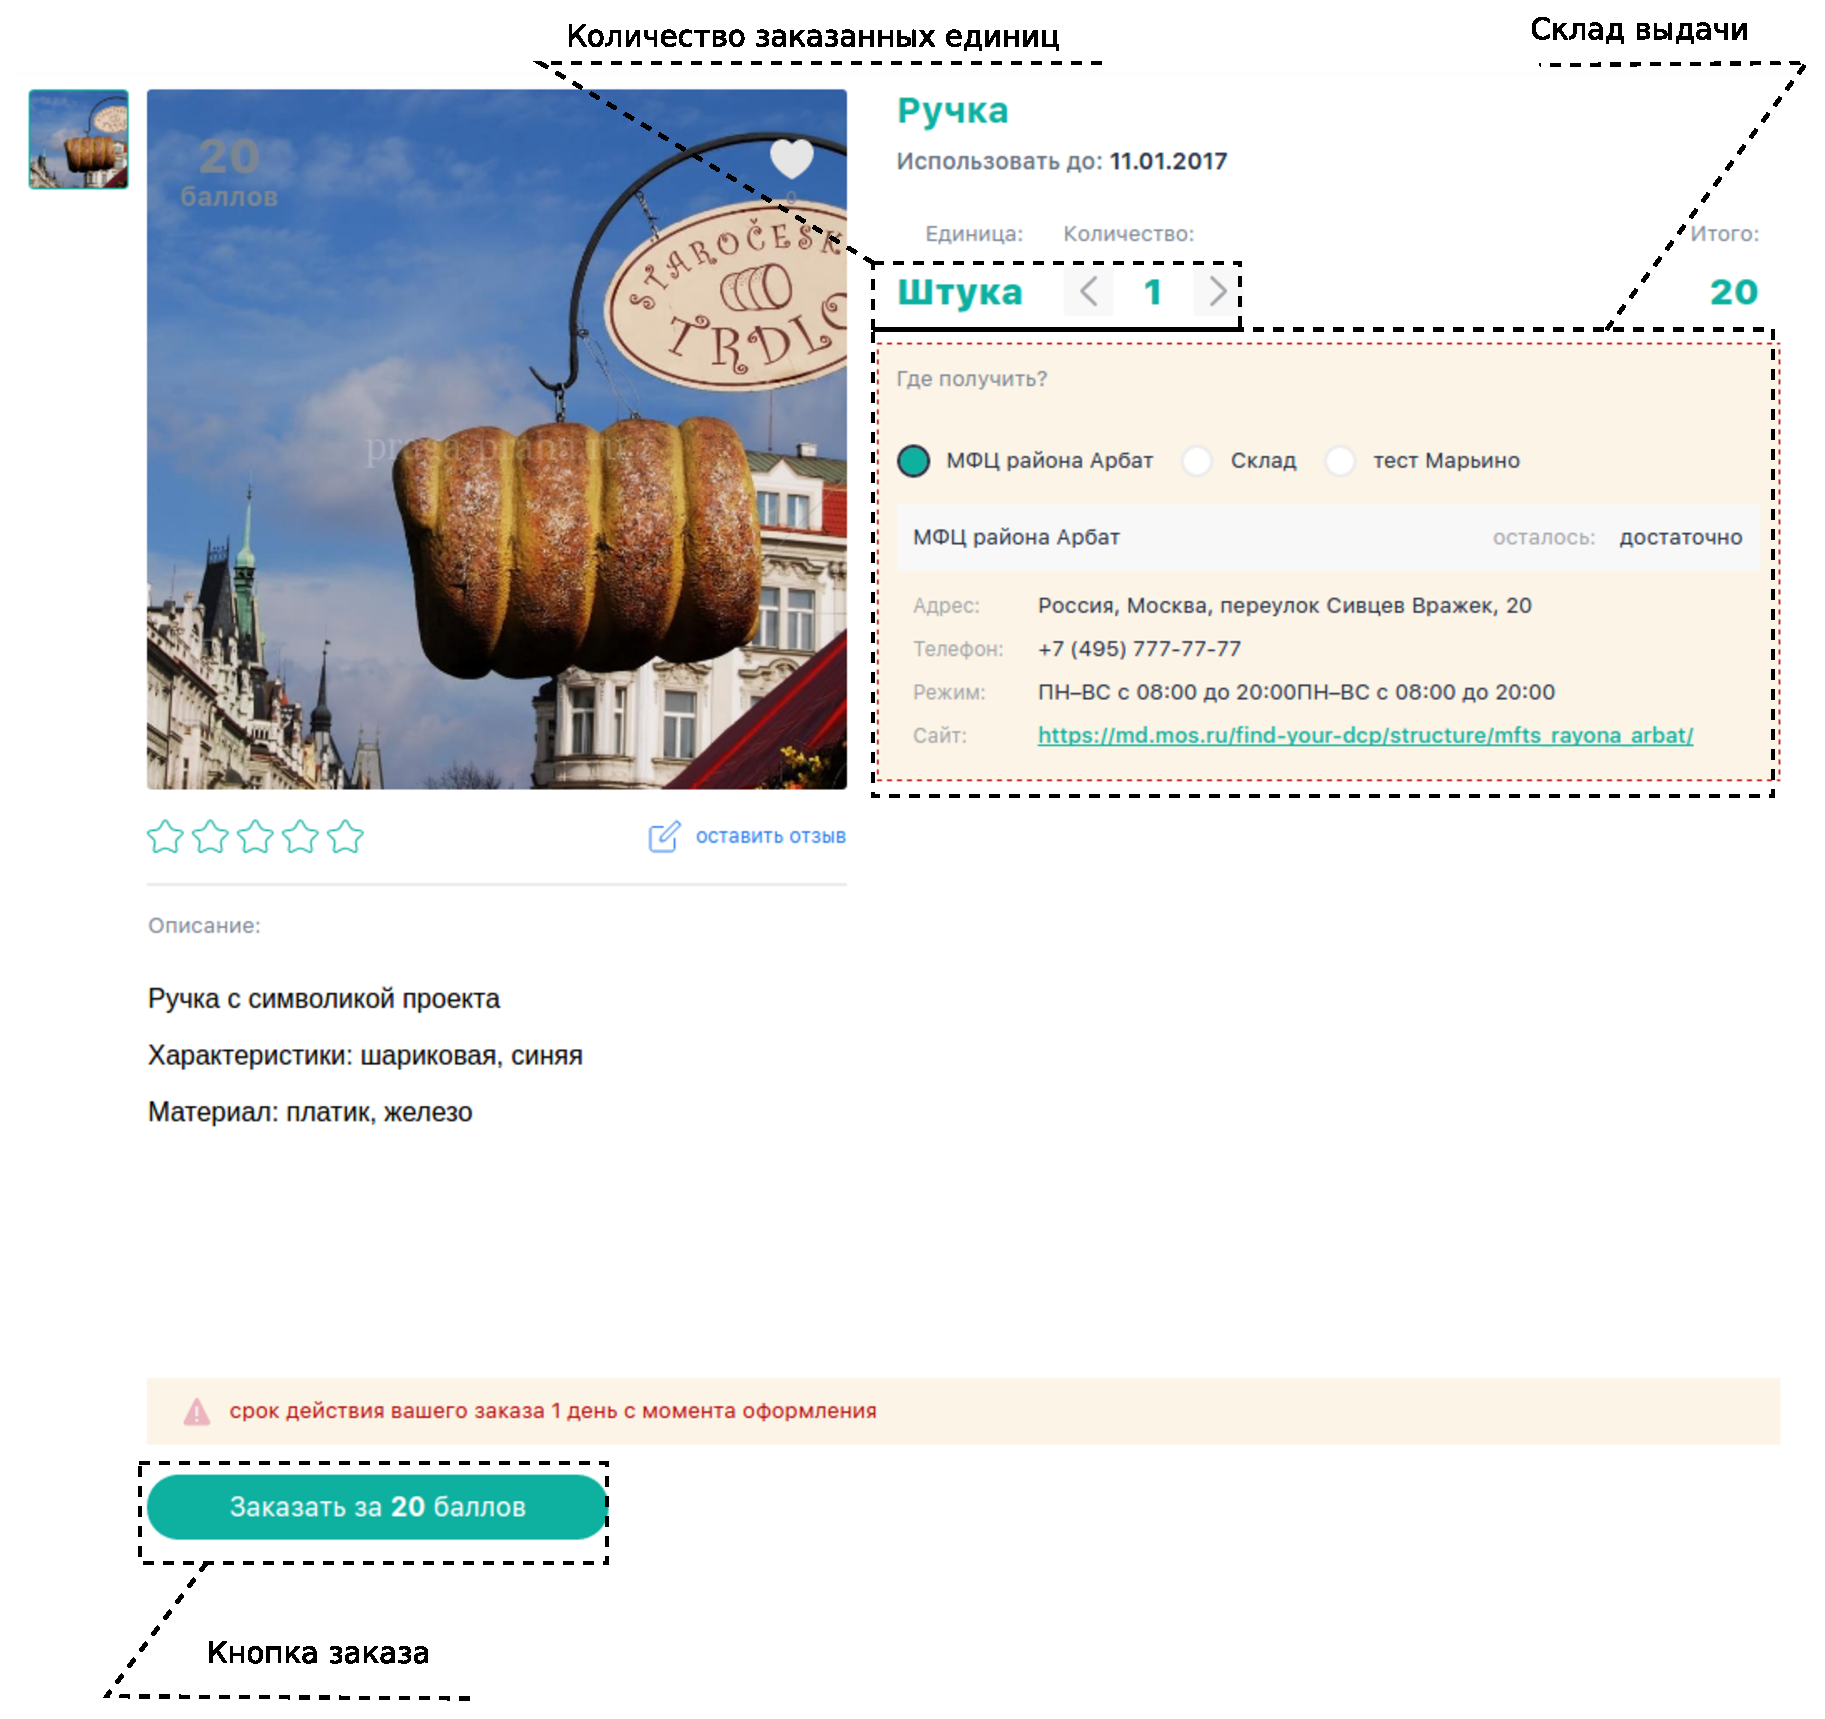
\includegraphics[width=170mm]{04_auth_funcs/figures/05.eps}
                \caption{Карточка товара для авторизованного пользователя}
                \label{fig:auth_goods_cart}
            \end{figure}
                
            \begin{figure}
                \center
                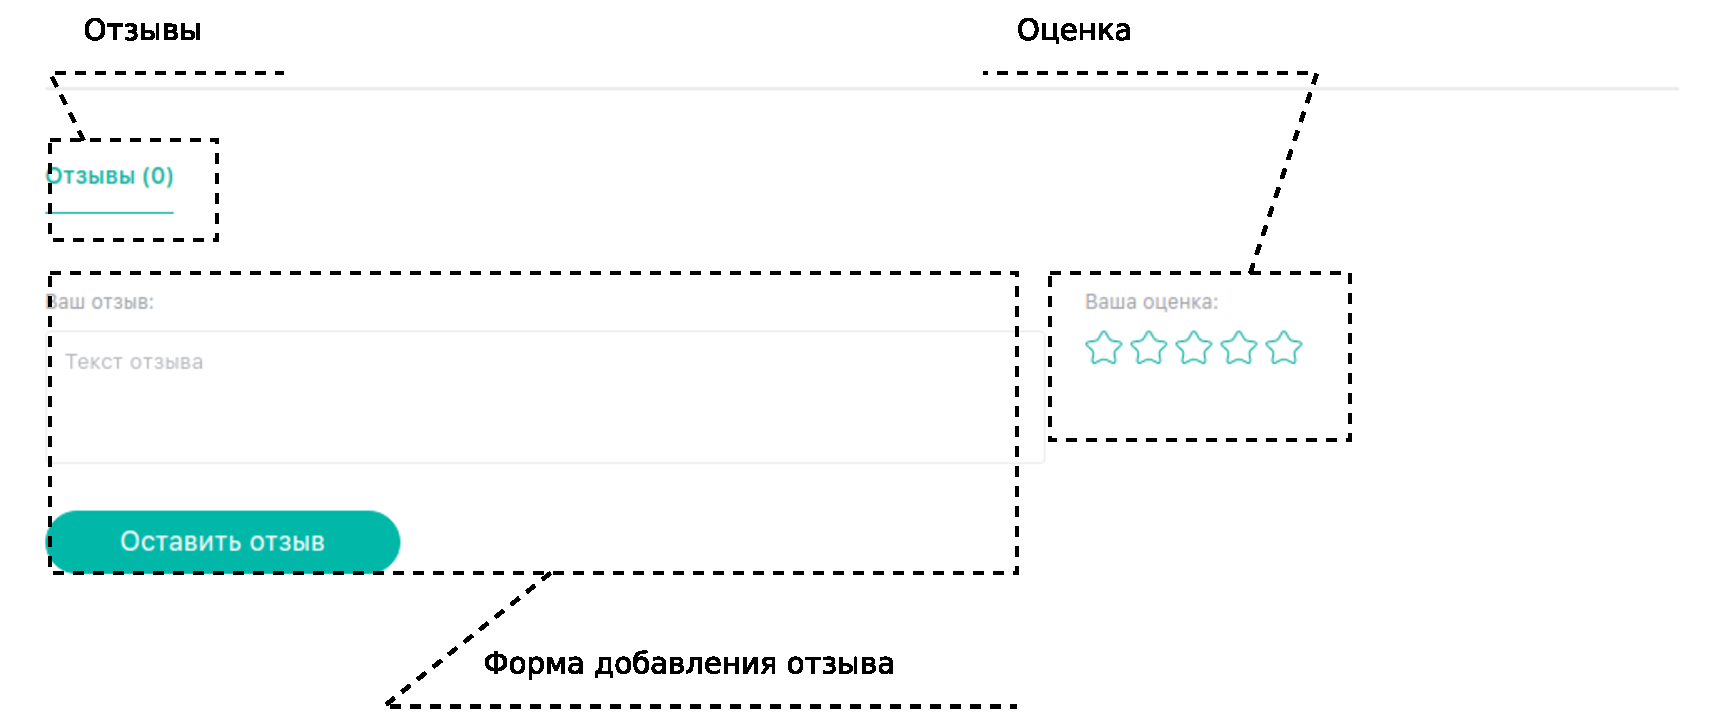
\includegraphics[width=170mm]{04_auth_funcs/figures/06.eps}
                \caption{Добавление отзыва для авторизованного пользователя}
                \label{fig:auth_goods_cart_otz}
            \end{figure}

                
     \section{Профиль пользователя}

        \subsection{Мои заказы}
        
            См. рис. \ref{fig:auth_my_orders}
     
        
            \subsubsection{Вкладка <<могу использовать>>}
            \subsubsection{Вкладка <<уже использовал>>}
            \subsubsection{Вкладка <<все заказы>>}
            \subsubsection{Карточка заказа}
                \paragraph{Номер заказа}
                \paragraph{Дата заказа}
                \paragraph{Статус заказа}
                \paragraph{Печать сертификата}
                \paragraph{Связь с администрацией}
                \paragraph{Отмена заказа}
                \paragraph{Фото товара}
                \paragraph{Стоимость заказа}
                \paragraph{Название товара}
                \paragraph{Склад}
                \paragraph{Переход к форме отзыва}
                \paragraph{Количество заказанных единиц}
                \paragraph{Цена товара}
            
        \subsection{Мои баллы}

            См. рис. \ref{fig:auth_my_points}
        
            \subsubsection{Дата}
            \subsubsection{Операция}
            \subsubsection{Баллы}
            \subsubsection{Пагинация}
            
        \subsection{Мои желания}
            \label{sec:auth_my_wishes}
            См. рис. \ref{fig:auth_my_wishes}
        
        
        